
\documentclass[a4paper,11.5pt]{article}
\usepackage[textwidth=170mm, textheight=230mm, inner=20mm, top=20mm, bottom=30mm]{geometry}
\usepackage[normalem]{ulem}
\usepackage[utf8]{inputenc}
\usepackage[T1]{fontenc}
\PassOptionsToPackage{defaults=hu-min}{magyar.ldf}
\usepackage{pgfplots}
\pgfplotsset{compat=1.10}
\usepgfplotslibrary{fillbetween}
\usepackage[magyar]{babel}
\usepackage{amsmath, amsthm,amssymb,paralist,array, ellipsis, graphicx, float, bigints,tikz}
%\usepackage{marvosym}

\makeatletter
\renewcommand*{\mathellipsis}{%
	\mathinner{%
		\kern\ellipsisbeforegap%
		{\ldotp}\kern\ellipsisgap
		{\ldotp}\kern\ellipsisgap%
		{\ldotp}\kern\ellipsisaftergap%
	}%
}
\renewcommand*{\dotsb@}{%
	\mathinner{%
		\kern\ellipsisbeforegap%
		{\cdotp}\kern\ellipsisgap%
		{\cdotp}\kern\ellipsisgap%
		{\cdotp}\kern\ellipsisaftergap%
	}%
}
\renewcommand*{\@cdots}{%
	\mathinner{%
		\kern\ellipsisbeforegap%
		{\cdotp}\kern\ellipsisgap%
		{\cdotp}\kern\ellipsisgap%
		{\cdotp}\kern\ellipsisaftergap%
	}%
}
\renewcommand*{\ellipsis@default}{%
	\ellipsis@before
	\kern\ellipsisbeforegap
	.\kern\ellipsisgap
	.\kern\ellipsisgap
	.\kern\ellipsisgap
	\ellipsis@after\relax}
\renewcommand*{\ellipsis@centered}{%
	\ellipsis@before
	\kern\ellipsisbeforegap
	.\kern\ellipsisgap
	.\kern\ellipsisgap
	.\kern\ellipsisaftergap
	\ellipsis@after\relax}
\AtBeginDocument{%
	\DeclareRobustCommand*{\dots}{%
		\ifmmode\@xp\mdots@\else\@xp\textellipsis\fi}}
\def\ellipsisgap{.1em}
\def\ellipsisbeforegap{.05em}
\def\ellipsisaftergap{.05em}
\makeatother

\usepackage{hyperref}
\hypersetup{
	colorlinks = true	
}

\DeclareMathOperator{\Int}{int}
\DeclareMathOperator{\tg}{tg}
\DeclareMathOperator{\ctg}{ctg}
\DeclareMathOperator{\sign}{sign}
\DeclareMathOperator{\Th}{th}
\DeclareMathOperator{\sh}{sh}
\DeclareMathOperator{\ch}{ch}
\DeclareMathOperator{\arsh}{arsh}
\DeclareMathOperator{\arch}{arch}
\DeclareMathOperator{\arth}{arth}
\DeclareMathOperator{\arcth}{arcth}
\DeclareMathOperator{\grad}{grad}
\DeclareMathOperator{\arc}{arc}
\DeclareMathOperator{\arctg}{arc tg}
\DeclareMathOperator{\arcctg}{arc ctg}
\newcommand{\norm}[1]{\left\lVert#1\right\rVert}

\begin{document}
	%%%%%%%%%%%RÖVIDÍTÉSEK%%%%%%%%%%
	\setlength\parindent{0pt}
	\def\a{\textbf{a}}
	\def\b{\textbf{b}}
	\def\N{\hskip 10 true mm}
	\def\a{\textbf{a}}
	\def\b{\textbf{b}}
	\def\c{\textbf{c}}
	\def\d{\textbf{d}}
	\def\e{\textbf{e}}
	\def\gg{$\gamma$}
	\def\vi{\textbf{i}}
	\def\jj{\textbf{j}}
	\def\kk{\textbf{k}}
	\def\fh{\overrightarrow}
	\def\l{\lambda}
	\def\m{\mu}
	\def\v{\textbf{v}}
	\def\0{\textbf{0}}
	\def\s{\hspace{0.2mm}\vphantom{\beta}}
	\def\Z{\mathbb{Z}}
	\def\Q{\mathbb{Q}}
	\def\R{\mathbb{R}}
	\def\C{\mathbb{C}}
	\def\N{\mathbb{N}}
	\def\Rn{\mathbb{R}^{n}}
	\def\Ra{\overline{\mathbb{R}}}
	\def\sume{\displaystyle\sum_{n=1}^{+\infty}}
	\def\sumn{\displaystyle\sum_{n=0}^{+\infty}}
	\def\biz{\emph{Bizonyítás:\ }}
	\def\narrow{\underset{n\rightarrow+\infty}{\longrightarrow}}
	\def\limn{\displaystyle\lim_{n\to +\infty}}
	%	\def\definition{\textbf{Definíció:\ }}
	%	\def\theorem{\textbf{Tétel:\ }}
	%\def\note{\emph{Megjegyzés:\ }}
	%\def\example{\textbf{Példa:\ }} 
	
	\theoremstyle{definition}
	\newtheorem{theorem}{Tétel}[subsubsection]
	
	\theoremstyle{definition}
	\newtheorem{definition}[theorem]{Definíció}
	\newtheorem{example}[theorem]{Példa}
	\newtheorem{exercise}[theorem]{Házi feladat}
	\newtheorem{note}[theorem]{Megjegyzés}
	\newtheorem{task}[theorem]{Feladat}
	\newtheorem{revision}[theorem]{Emlékeztető}
	%%%%%%%%%%%%%%%%%%%%%%%%%%%%%%%%%
	\begin{center}
		{\LARGE\textbf{Az analízis alkalmazásai}}
		\smallskip

		{\Large Gyakorlati jegyzet}

		\smallskip
		2. óra.
	\end{center}
	A jegyzetet \textsc{Umann} Kristóf készítette \textsc{Kovács} Sándor gyakorlatán. (Utoljára frissítve: \today)
	
	\section{Többváltozós integrál (folyt.)}
	\begin{theorem}
		$T\subset \R^N$ tégla $\overset{(\tau\in\mathcal{F}(T))}{\rightsquigarrow}\quad T_1,\ldots,T_n$ résztéglára bomlik
		\[f\in R(T)\quad \Rightarrow\quad \forall k:\quad f_{\big|_{T_k}}\in R(T_k)\quad (f\in R(T_k))\quad \text{és}\quad  \int_{T}f=\sum_{k=1}^n\int_{T_k}f \]
	\end{theorem}
	\begin{definition}
		$T\subset\R^M, S\subset\R^N$ tégla, $f:T\times S\to\R,$
		\[ \forall r\in T:\quad f_r:S\to\R,\quad f_r(s):=f(r,s) \]
		\[ \forall s\in S:\quad f^s:T\to\R,\quad f^s(r):=f(r,s) \]
	\end{definition}
	\begin{theorem}
		$T\subset \R^N$ tégla: $C(T)\subset R(T)$
	\end{theorem}
	\begin{theorem}
		(Fubini) $f: T\times S\to\R$ korlátos fv., $f\in R(T\times S)$. 
		
		\smallskip
		1. Ha $\forall r\in T:\quad f_r\in R(S)\Rightarrow T\ni r\to\int_Sf_r(s)\,ds$\quad Riemann integrálható, és
		\[ \int_{T\times S}f=\int_T\left(\int_Sf_r(s)\,ds\right)\,dr=\int_T\left(\int_Sf(r,s)\,ds\right)\,dr \]
		
		\smallskip
		1. Ha $\forall s\in S:\quad f^s\in R(S)\Rightarrow S\ni s\to\int_Sf_r(r)\,dr$ Riemann integrálható, és
		\[ \int_{T\times S}f=\int_S\left(\int_Tf^s(r)\,dr\right)\,ds=\int_S\left(\int_Tf(r,s)\,dr\right)\,ds \]
		
	\end{theorem}
	\begin{example}
		$T:=[0,1]\times[-1,2]$
		\[ f(x,y):=x^2y\quad ((x,y)\in T)\]
		$\forall r\in[0,1],\quad f_r(s):=r^2s\quad (s\in[-1,2])\quad \Rightarrow\quad f_r\in C[-1,2]\quad \Rightarrow\quad f_r\in R[-1,2]$ \quad és \[\int_{-1}^{2}f_r(s)\,ds=\int_{-1}^{2}r^2s\,ds=r^2\left[\frac{s^2}{2}\right]_{-1}^2=\frac{3r^2}{2}, \quad f\in R([0,1]\times[-1,2])\]
		\[ \Rightarrow\quad \int_{[0,1]\times[-1,2]}^{}f=\int_{0}^{1}\left(\int_{-1}^{2}f(r,s)\,ds\right)=\frac{3}{2}\left[\frac{r^3}{3}\right]^1_0=\frac{1}{2} \]
	\end{example}
	\begin{theorem}
		$f\in R[a,b],\quad g\in R[c,d],\quad F:[a,b]\times[c,d]\to\R,\quad F(x,y):=f(x)g(y)$
		\[ \Rightarrow\quad F\in R([a,b]\times[c,d])\quad \text{és}\quad \int_{[a,b]\times[c,d]}^{}F=\left(\int_{a}^{b}f\right)\left(\int_{c}^{d}g\right) \]
	\end{theorem}
	\begin{example}
		$F(x,y):=x^2y,\quad ((x,y)\in[0,1]\times[-1,2])\quad \Rightarrow\quad F\in R([0,1]\times[-1,2])$
		\[ \Rightarrow\quad \int_{[0,1]\times[-1,2]}F=\left(\int_{0}^{1}x^2\,dx\right)\left(\int_{-1}^{2}y\,dy\right)=\left[\frac{x^3}{3}\right]_0^1 \left[\frac{y^2}{2}\right]_1^2=\frac{1}{3}\cdot\frac{3}{2}=\frac{1}{2} \]
	\end{example}
	\begin{definition}
		$H\subset\R^N$ korlátos halmaz, $H\subset T\subset\R^N$ tégla, $f:H\to\R$ korlátos fv., $\tilde{f}:T\to\R,$
		\[ \quad \tilde{f}(r):=\begin{cases}
			f(r)\quad (r\in H)\\
			0\quad (r\in T\setminus H)
		\end{cases} \]
		Azt mondjuk hogy $f\in R(H)$, ha $\tilde{f}\in R(T)$ és ez utóbbi esetben 
		\[ \int_Hf:=\int_T\tilde{f} \]
	\end{definition}
	\begin{definition}
		Adott az $\varOmega\subset \R^2$ halmaz,
		\begin{enumerate}
			\item \emph{normáltartomány az $x$-tengelyre vonatkozóan}, ha
			\[ \exists\varphi,\psi \in C[a,b]:\quad \varphi\leq\psi \quad \text{és}\quad \varOmega=\{(x,y)\in\R^2:\quad x\in[a,b],\quad y\in[\varphi(x),\psi (y)] \}\]
			\item \emph{normáltartomány az $y$-tengelyre vonatkozóan}, ha
			\[ \exists\mu,\nu\in C[c,d]:\quad \mu\leq\nu\quad \text{és}\quad \varOmega=\{(x,y)\in\R^2:\quad y\in[c,d],\quad x\in[\mu(x),\nu(y)] \}\]
			\item \emph{krumpli}, ha normáltartomány mind az $x$, mind pedig az $y$ tengelyre vonatkozóan.
		\end{enumerate}
	\end{definition}
	\begin{theorem}
		$K,H\subset\R^2$ normáltartomány az $x$, és az $y$ tengelyre vonatkozóan,\quad $f:K\to\R,$ $f\in C$,\quad $g:H\to \R;$ $g\in C$
		\[ \Rightarrow\quad \int_K f=\int_{a}^{b}\left(\int_{\varphi(x)}^{\psi (x)}f(x,y)\,dy\right)\,dx\quad \text{és}\quad \int_Hg=\int_{c}^{d}\left(\int_{\mu(y)}^{\nu(y)}g(x,y)\,dx\right)\,dy \]
	\end{theorem}
	\begin{task}
		\[ \int_0^2\left(\int_{y^4}^4y\cdot\ch\left(x^2\right)\,dx \right)\,dy=? \]
		Ezt átírhatjuk az előző tétel alapján:
		\[ \int_{\varOmega}^{}f(x,y)\,d(x,y), \]
		ahol 
		\[ \varOmega=\{(x,y)\in\R^2:\quad y\in[0,2], \quad x\in[y^2,4]\},\quad f(x,y):=y\ch\left(x^2\right)\quad (x,y)\in\varOmega  \]
		\begin{figure}[h]
			\centering
			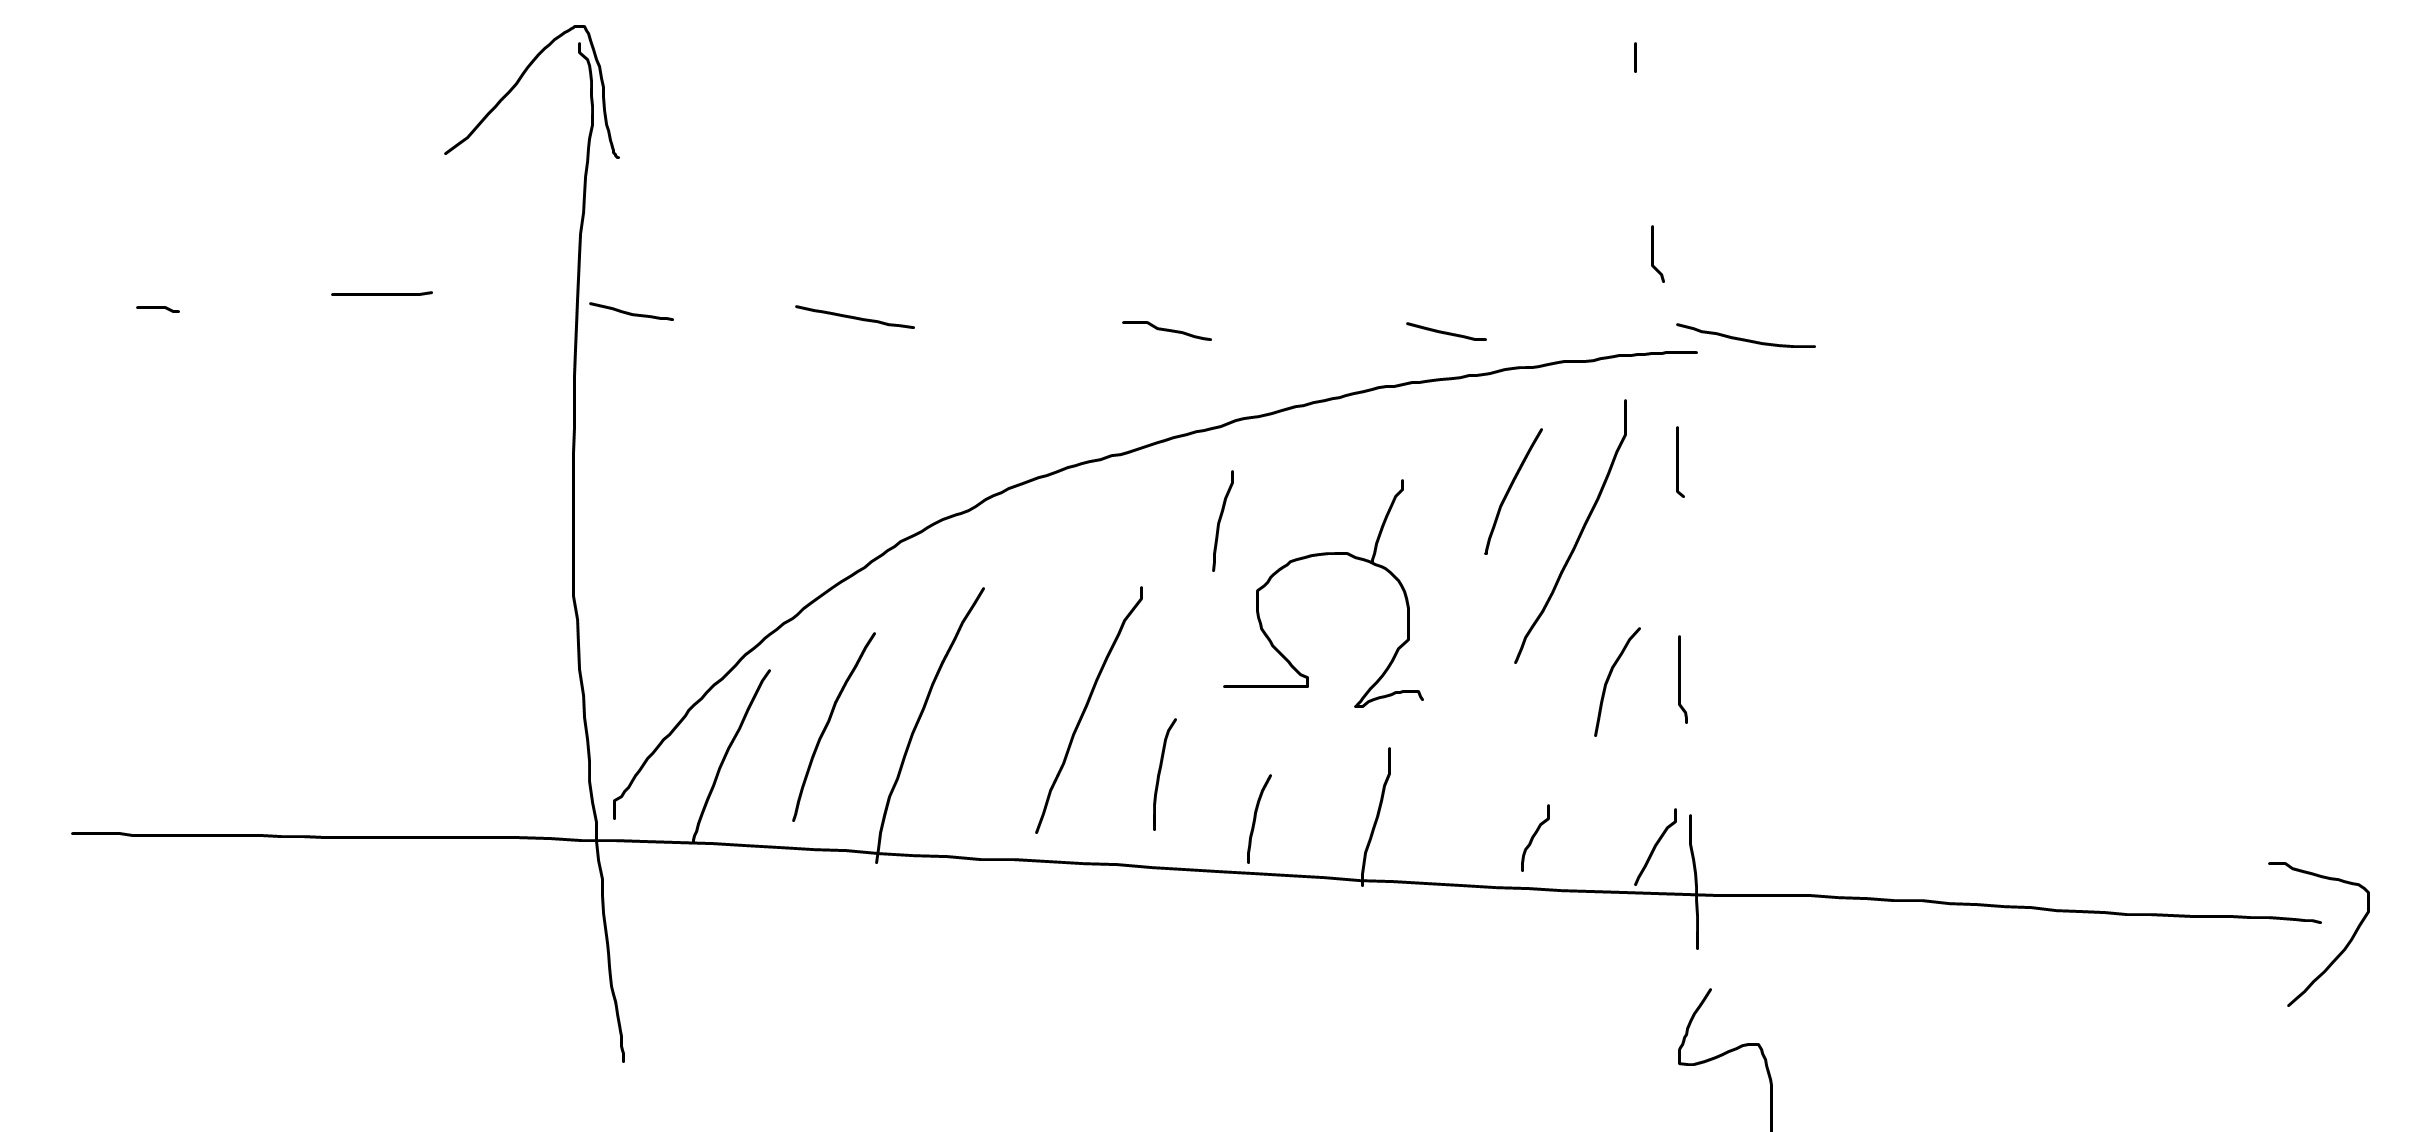
\includegraphics[width=7cm]{kepek/01.png}
			\caption{}
		\end{figure}
		\[ \Rightarrow \quad \int_{\varOmega}^{}f=\int_0^4\left(\int_{0}^{\sqrt{x}}y\ch\left(x^2\right)\,dy\right)\,dx=\int_{0}^{4}\left[\frac{y^2}{2}\ch\left(x^2\right)\right]_{y=0}^{y=\sqrt{x}}\,dx=\frac{1}{4}\int_0^42x\ch\left(x^2\right)\,dx=\frac{1}{4}\left[\sh\left(x^2\right)\right]_0^4=\frac{\sh(16)}{4} \]
	\end{task}
	\begin{definition}
		Azt mondjuk, hogy $H\subset\R^N$ Jordan-mérhető, ha $\exists H\subset T\subset\R^N$ tégla:
		\[ \mathcal{X}_H:T\to\R,\quad \mathcal{X}_H(r):=\begin{cases}
			1\quad (r\in H)\\
			0\quad (r\in T\setminus H)
		\end{cases}\quad \text{fv.-re}\quad \mathcal{X}_H\in R(T)\]
		és $H$ mértéke
		\[ |H|=\int_T\mathcal{X}_H=\int_H1. \]
	\end{definition}
	\begin{note}\ 
		
		\begin{enumerate}
			\item $T\subset\R^N$ tégla\quad$\quad \Rightarrow\quad T$ Jordan mérhető és $|T|=\mu(T)$
			\item $N=2:\quad |H|:\ H$ területe, $N=3:\quad H:\ H$ térfogata 
		\end{enumerate}
	\end{note}
	\begin{theorem}
		(Helyettesítéses integrálás)  $d\in\N,\quad U\subset\R^d$ nyílt, $\phi:U\to\R^d$ injektív, folyamatosan differenciálható:\quad $\det[\varphi'(r)]\not=0\quad (r\in U)$. 
		
		Ha $K\subset U$ kompakt és Jordan-mérhető, akkor $\phi[k]$ Jordan-mérhető, és
		\[ |\phi[k]|=\int_K|\det[\phi'(r)]|\,dr. \]
		 Sőt, ha $f:\phi[k]\to\R,\quad f\in C$
		 \[ \Rightarrow\quad \int_{\phi[k]}f=\int_Kf(\phi(r))\cdot\big|\det[\phi'(r)]\big|\,dr \]
	\end{theorem}
	\begin{note}\
		
		$N\subset K:\quad |N|=0\quad \Rightarrow\quad$ lehet:
		\begin{itemize}[$\bullet$]
			\item $\det[\phi'(r)]=0\quad (r\in\N)$
			\item $\phi_{\big|_N}$ nem injektív
		\end{itemize}
	\end{note}
\end{document}